% Figure snippets generated by plot-agent. All numeric values trace to
% inputs/experimental_log.md. Embed inline in main.tex rather than \input{}.

% Figure: experimental setup schematic
\begin{figure}[htbp]
\centering
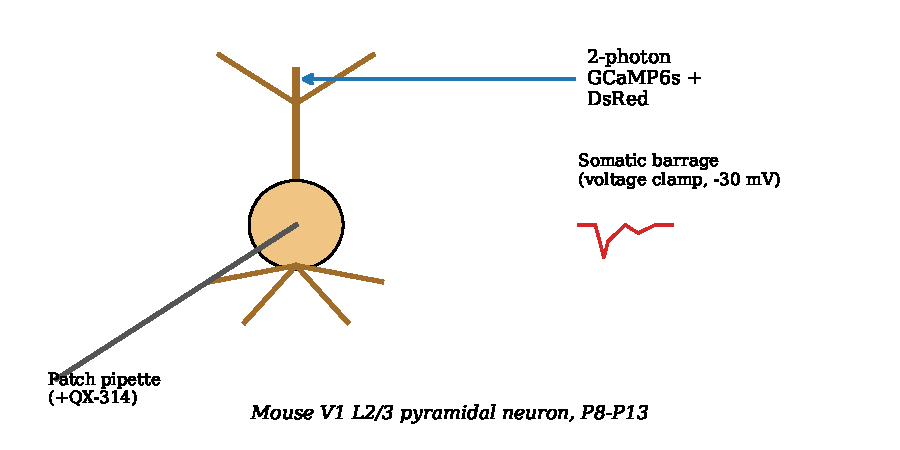
\includegraphics[width=0.75\textwidth]{figures/fig_setup_schematic.pdf}
\caption{Experimental configuration. Layer 2/3 pyramidal neurons in the mouse primary visual cortex were targeted in vivo for whole-cell voltage-clamp recording under two-photon guidance. GCaMP6s and DsRed were delivered by in utero electroporation at embryonic day 16.5; QX-314 in the internal solution blocked somatic action potentials. Holding the neuron at $-30$ mV facilitated NMDA-receptor-dependent calcium transients at both spine and shaft synapses.}
\label{fig:setup}
\end{figure}

% Figure: transmission rates spine vs shaft at two ages
\begin{figure}[htbp]
\centering
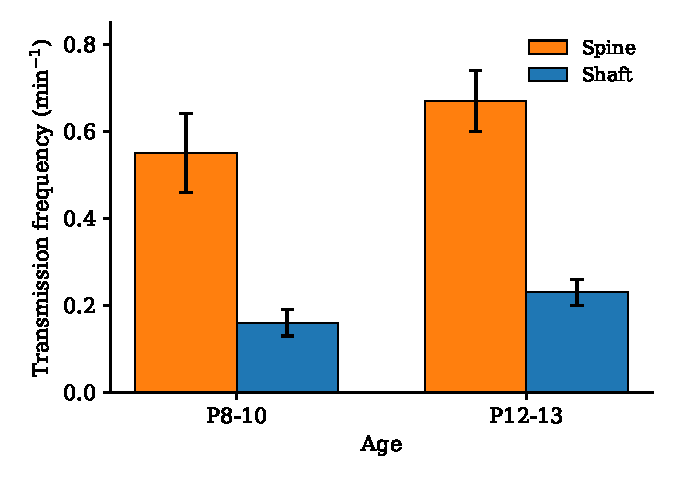
\includegraphics[width=0.55\textwidth]{figures/fig_transmission_rates.pdf}
\caption{Spine synapses sustained higher transmission rates than shaft synapses at both developmental stages (P8--10: spine $0.55 \pm 0.09$ min$^{-1}$ vs.\ shaft $0.16 \pm 0.03$ min$^{-1}$; P12--13: spine $0.67 \pm 0.07$ min$^{-1}$ vs.\ shaft $0.23 \pm 0.03$ min$^{-1}$; mean $\pm$ SEM; each $p < 10^{-9}$, Mann--Whitney $U$ test; P8--10 $n = 36$ spine and $113$ shaft, P12--13 $n = 83$ spine and $122$ shaft).}
\label{fig:rates}
\end{figure}

% Figure: domain features
\begin{figure}[htbp]
\centering
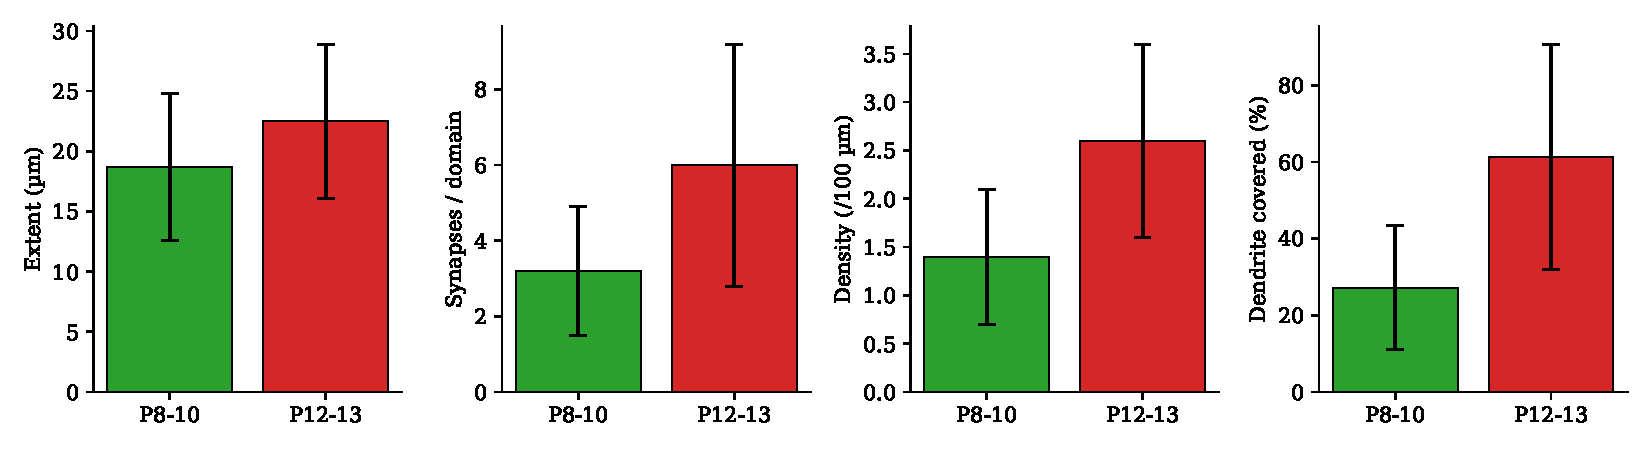
\includegraphics[width=0.95\textwidth]{figures/fig_domain_features.pdf}
\caption{Dendritic domains grew on four axes during the second postnatal week. Extent increased modestly (P8--10: $18.7 \pm 6.1$ $\mu$m; P12--13: $22.5 \pm 6.4$ $\mu$m), while synapses per domain (P8--10: $3.2 \pm 1.7$; P12--13: $6.0 \pm 3.2$) and domain density along dendrites (P8--10: $1.4 \pm 0.7$; P12--13: $2.6 \pm 1.0$ per 100 $\mu$m) approximately doubled. The fraction of dendritic length covered by domains rose from $27.2 \pm 16.2\%$ to $61.3 \pm 29.4\%$ (mean $\pm$ STD).}
\label{fig:domains}
\end{figure}

% Figure: in-domain vs out-of-domain co-activity
\begin{figure}[htbp]
\centering
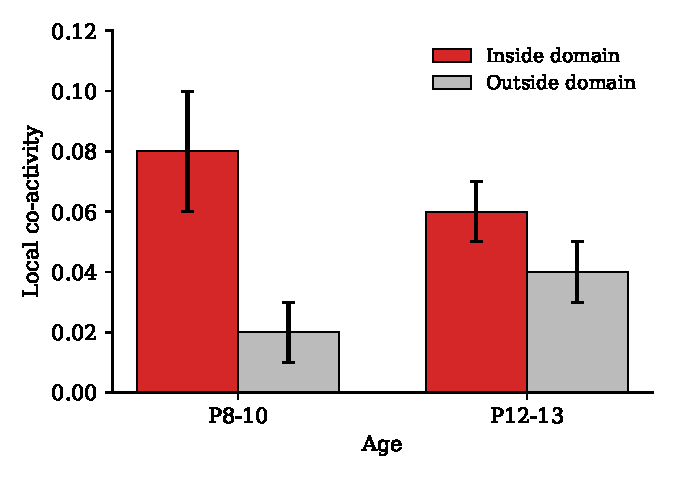
\includegraphics[width=0.55\textwidth]{figures/fig_coactivity.pdf}
\caption{Local co-activity was consistently higher inside than outside dendritic domains at both ages (P8--10: in-domain $0.08 \pm 0.02$, out-of-domain $0.02 \pm 0.01$; P12--13: in-domain $0.06 \pm 0.01$, out-of-domain $0.04 \pm 0.01$; mean $\pm$ SEM; $n = 213$ in-domain, $173$ out-of-domain synapses; Mann--Whitney $U$ test).}
\label{fig:coactivity}
\end{figure}

% Figure: model of domain formation
\begin{figure}[htbp]
\centering
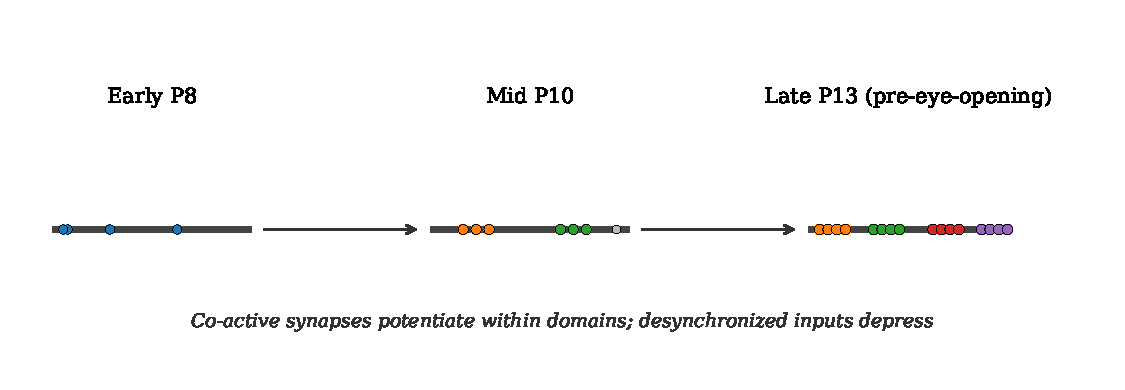
\includegraphics[width=0.95\textwidth]{figures/fig_domain_schematic.pdf}
\caption{Model of dendritic-domain assembly before eye opening. At P8, only a few active synapses are scattered across the developing dendrite. During the second postnatal week, synapses sort into functionally distinct domains: in-sync synapses stabilize or potentiate while desynchronized inputs undergo depression. By P12--13, dendrites are largely covered by domains of neighbors whose co-activity within a domain exceeds co-activity across domains.}
\label{fig:model}
\end{figure}
